\documentclass[11pt]{article}

\usepackage{inputenc}
\usepackage{graphicx}
\usepackage[sort&compress,super]{natbib}
\citestyle{naturemag}
\usepackage{sgame}
\usepackage{amssymb,amsmath}
%\usepackage[nolists]{endfloat}
\usepackage[pdfborder={0 0 0}]{hyperref}
\usepackage{chngpage}
\usepackage{pdflscape}
\usepackage{epstopdf}
\usepackage{fullpage}
\usepackage{setspace}
\usepackage{booktabs}
\usepackage{dcolumn}
\usepackage{subfigure}
\usepackage{ae,aecompl}
\usepackage[T1]{fontenc}
\usepackage{array}

\subfigcapmargin = 0.1cm

\usepackage{xr-hyper}
\usepackage{hyperref}
\externaldocument{Stacking}

\makeatletter
\newcommand{\noun}[1]{\textsc{#1}}

\renewcommand{\thefigure}{A\arabic{figure}}
\renewcommand{\thetable}{A\arabic{table}}
\renewcommand{\refname}{Supporting Information: References}

\renewcommand{\thesection}{A\arabic{section}}
\renewcommand{\thesubsection}{A\arabic{section}.\arabic{subsection}}
\renewcommand{\thesubsubsection}{A\arabic{section}.\arabic{subsection}.\arabic{subsubsection}}

\bibpunct{}{}{,}{s}{}{}

\renewcommand{\thepage}{APP-\arabic{page}}

%%%%%%%%%%%%%%%%%%%%%%%%%%%%%% LyX specific LaTeX commands.
%% Because html converters don't know tabularnewline
\providecommand{\tabularnewline}{\\}

%% A simple dot to overcome graphicx limitations

\newcommand{\lyxdot}{.}
\begin{document}

\title{Jointly Modeling the Adoption, Consumption, and Exclusive Use of Clean Cooking Fuels in Rural India\\\textbf{Supporting Information}}

\author{Carlos Gould\\Columbia University \and Xiaoxue Hou\\Johns Hopkins SAIS \and Jennifer Richmond\\University of Maryland \and Anjali Sharma\\University of Maryland \and Johannes Urpelainen\footnote{Corresponding author. Address: Rome Building, 4th Floor. 1619 Massachusetts Avenue, NW. Washington, DC 20036, USA. Tel: +1-734-757-0161. Email: JohannesU@jhu.edu.}\\Johns Hopkins SAIS}

\maketitle

\tableofcontents

\clearpage

\doublespacing

\section{Supplementary Note}
\label{sect:data}
\subsection{Data}
The Access to Clean Cooking Energy and Electricity -- Survey of States (ACCESS) is the largest energy access survey conducted in India. A total of 8,568 households in 2015 and 9,072 households in 2018 were sampled to evaluate energy and electricity patterns over time. The increase in sample size in the second wave is attributed to an addition of 504 households in three added districts in the state of Odisha to balance the sample distribution among states. The full listing, therefore, contains 17,640 sampled households. However, for the purposes of our analysis, only 8,563 households were able to be interviewed in 2015, and only a total of 9,008 observations are able to be used for 2018 because of missing data for specific, key variables needed to perform our estimations.

The survey was designed to take 40-45 minutes to administer per household. The median time to complete the survey in the first wave was 37 minutes. The questionnaire included the following modules: socioeconomic information, a household's current source(s) of electricity (if any), satisfaction with the electricity service, cooking fuel access, household energy policy preferences, and willingness to pay for LPG or electricity.

Sampling was done using a three-stage probability-proportional-to-size (PPS) survey design. Among six energy-deprived states (Bihar, Jharkhand, Madhya Pradesh, Odisha, Uttar Pradesh, and West Bengal), a total of 51 districts, 714 rural villages, and 17,640 households were sampled for each of the three stages. Due to practical constraints, only one district was sampled from each large administrative division within a state. The number of districts sampled per state is therefore proportional to the number of administrative divisions. This is true for each state except for Odisha in the second wave, which was oversampled to include three additional districts since there are fewer administrative divisions (three) compared to the other states. Using the 2011 Indian Census, villages were divided into small and large villages in each district based on population size to be able to distinguish any differences due to the size of the community. A total of 12 households were then sampled from each of the 714 rural villages among 51 districts. 

From 2015 to 2018, a total 86\% of the same households were interviewed in the second wave. Table \ref{t:retention} summarizes retention rates by study state. Households were identified by enumerators using a village listing. Enumerators requested heads of households to be interviewed, and if the head of the household was unavailable another willing adult was interviewed. If no adult in the household was available, or if the household was no longer willing to participate, enumerators replaced the household by interviewing the fifth household to the right of the originally sampled household. Enumerators were recruited and trained using role-playing exercises. 

\begin{table}
\centering
\renewcommand{\arraystretch}{1.8}
\begin{tabular}{lcr} % <-- Alignments: 1st column left, 2nd middle and 3rd right, with vertical lines in between
\textbf{State} & \textbf{Responses} & \textbf{Retention} \\
\hline
Bihar & 1,512 & 82\% \\
Jharkhand & 840 & 84\% \\
Madhya Pradesh & 1,680 & 77\% \\
Odisha & 1,008 & 82\% \\
Uttar Pradesh & 3,024 & 92\% \\ 
West Bengal & 1,008 & 88\% \\
\hline
\textbf{Total} & 9,072 & 86\% \\
\end{tabular}


\caption{Retention rates for the 2018 wave are shown here for household responses in each state. Note that only 504 households were sampled and interviewed in Odisha in 2015, and sampling for Odisha doubled to 1,008 for the 2018 wave; therefore, retention is based only on the 504 households from the first wave.}
\label{t:retention}
\end{table}

Questionnaires were designed to be easily understood and were tested and piloted in different settings to ensure that the instrument was effective. Regular quality checks were also done during data collection to ensure that data was coded correctly. Whereas paper questionnaires were used in 2015, digital questionnaires were used on tablets using the software program SurveyCTO for the 2018 wave. The digital survey program delivered regular, automated quality control reports, and it also made tracking the time and location of each survey more efficient. Finally, each respondent was briefed on the intent and purpose of the study as well as the nature of the questions before agreeing to participate. Written or oral consent was required from each respondent, depending on the respondent's writing ability. 

\clearpage

\section{Methods}
\label{sect:methods}
First, the generalized ordered logit model (\textbf{gologit model}) is denoted as the following equation, as elsewhere \citep{Williams2016}:

\begin{equation}
P(y_{it}>j)=\frac{exp(\alpha_{j} + X_{it} \beta_j + \Omega_{it}\beta n_{j})}{1+[exp(\alpha_{j} + X_{it} \beta_j + \Omega_{it} \beta n_{j})]}, j=2,3...,M-1
\end{equation}

where $P(y_{it}>j)$ is the probability that the household's $y$ outcome category is greater than $j$ in time period $t$, in which $j$ is the collapsed category of $j=1$, $j=1,2$, or $j=1,2,3$. The $\alpha$ intercept term captures fixed effects, and differs across values of $j$ to allow for different regression lines. $M$ is the number of categories, which is four in this case. $X_{it} \beta_j$ is the main explanatory variable, logged monthly expenditure for household $i$ in wave $t$ with an estimated coefficient that may vary across values of $j$. The term $\Omega_{it}\beta n_j$ includes a set of control variables, including number of household members, education, caste, female head of household, religion, and age. The estimated coefficients for the control variables may remain constant across values of $j$ or may vary across values of $j$ depending on whether each variable meets the parallel lines assumption in the stepwise application of Wald tests in the gologit2 package in Stata. Standard errors are clustered at the village level. Fixed effects are included for the state and the survey wave (2015 and 2018).

Second, our \textbf{double-hurdle model} is denoted by the following equation \citep{Garcia2013}:

\begin{equation}
\begin{split}
log(L) = \sum_{y_i = 0}^{} \Big[ log \Big\{ 1-\Phi \Big( z_i \gamma, \frac{x_i \beta}{\sigma}, \rho \Big) \Big\} \Big] + \sum_{y_i > 0}^{} \Big( log \Big[ \Phi \Big\{ \frac{z_i \gamma + \frac{\rho}{\sigma}(y_i-x_i\beta) }{\sqrt{1-\rho^2}} \Big\} \Big] 
\\
- log [\sigma] +log \Big\{ \phi \Big( \frac{y_i - x_i \beta}{\sigma} \Big) \Big\} \Big)
\end{split}
\end{equation}

where $y_i$ is either equal to $0$, which would exclude the observation to the selection stage, or $y_i > 0$, which would allow the observation to impact the second stage. The first stage excludes those households without access to LPG while elevating households with LPG access to the second stage to estimate levels of consumption. This is stated as the following restriction for the double hurdle model:

\begin{equation}
y_i = \left\{ \begin{array}{cl} x_i \beta + \epsilon_i & \textrm{if min} (x_i \beta +\epsilon_i, z_i\gamma+u_i) > 0 \\
0 & \textrm{otherwise} \end{array}\right.
\end{equation}

If households select out of the model in stage one, the model for these households is essentially the same as the log likelihood function of a tobit model. For households that enter into the second stage, additional parameters are added to the tobit model to estimate the continuous outcome of LPG consumption.

\clearpage

\section{Suppementary Figures}
\label{sect:robustness}

\begin{figure}[h!]
\centering
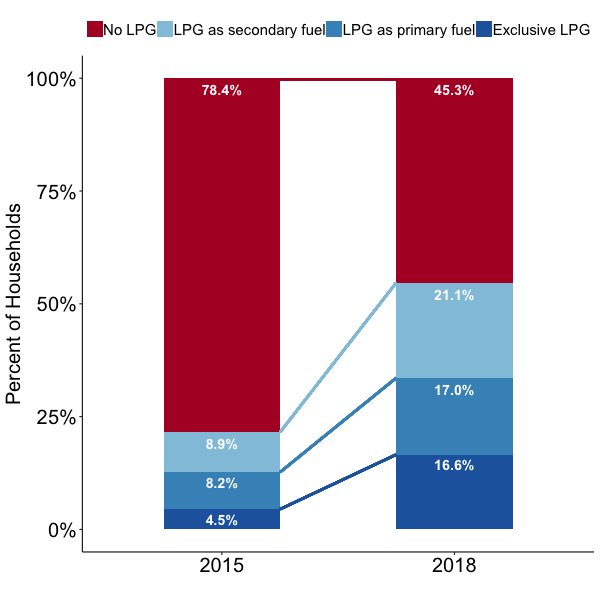
\includegraphics[scale=0.66]{Figures/Descriptive_Statistics/LPGCategories20152018.png}
\caption{Shifts in cooking fuel stacking patterns from ACCESS I (2015) to ACCESS II (2018).}
\label{bar_fuel_stack}
\end{figure}


\begin{figure}[h!]
\centering
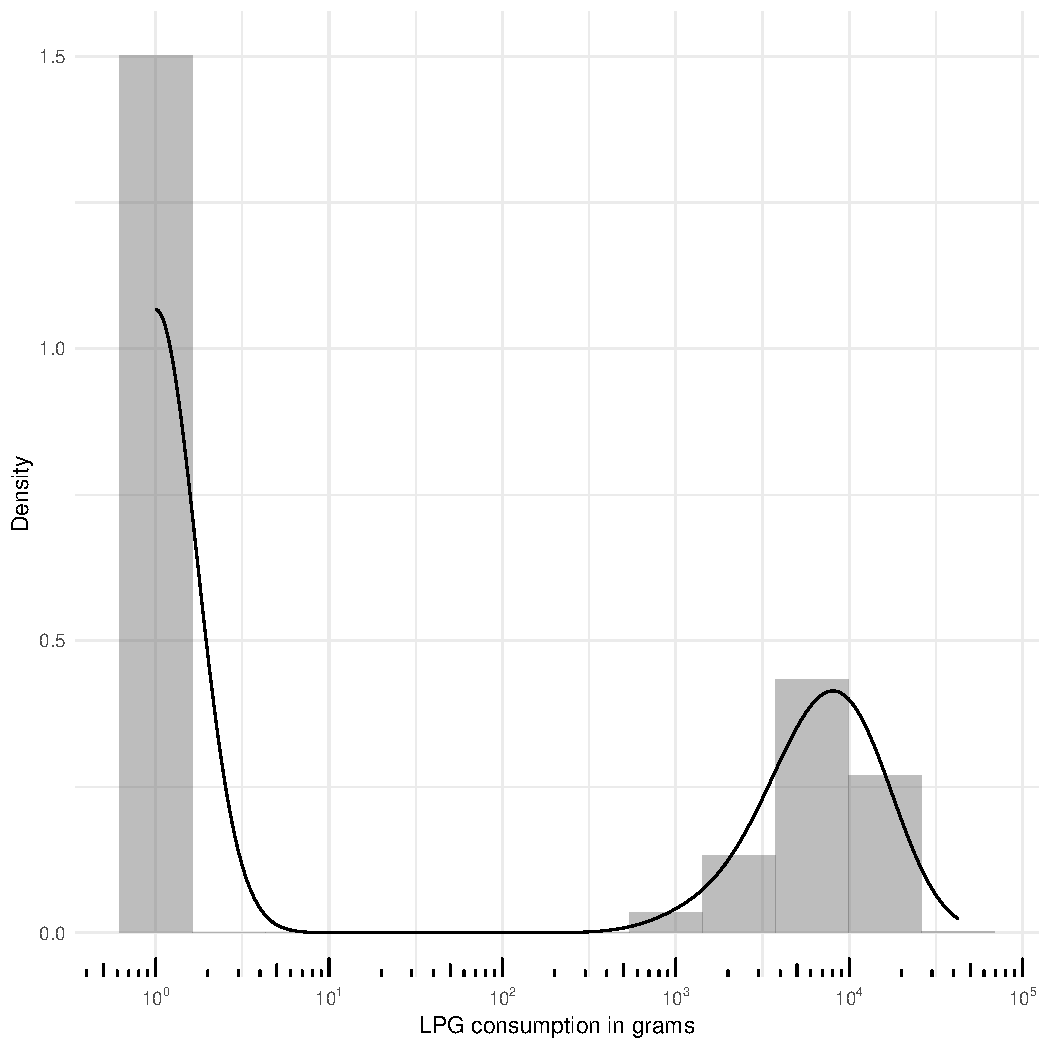
\includegraphics[scale=1]{Figures/Descriptive_Statistics/distribution_lpg_log.pdf}
\caption{Distribution of household LPG consumption in the study sample. We use logarithmic scale axes and transform the data by plus one accordingly. This figure shows a zero-inflated distribution and a near-normal distribution of our dependent variable. It gives intuitions on using two-stage regression to model household consumption of LPG. The first part is a binary logit model to predict the selection of LPG and the second part is a truncated Poisson model to predict the consumption of LPG.}
\label{distribution_lpg_log}
\end{figure}



\begin{figure}[h!]
	\centering
	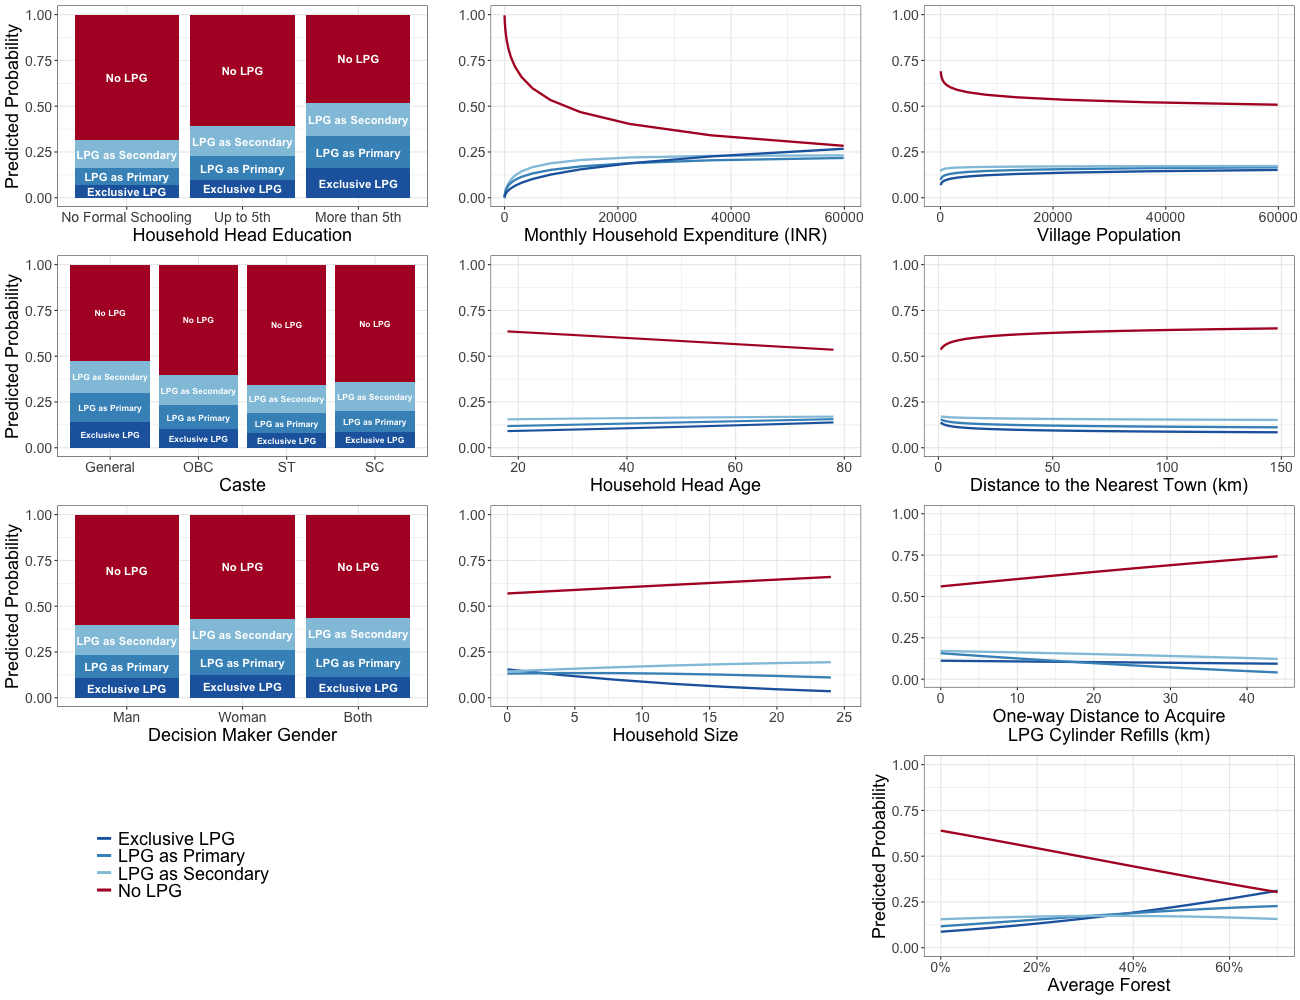
\includegraphics[scale=0.38]{Figures/Marginal_Effects/gologit_village.png}
\caption{\textbf{Predicted probability of fuel stacking category from generalized ordered logit model with village-level covariates.} Figure shows the comparison of predicted probability (0-1) of four levels of LPG adoption: exclusive LPG use, LPG as primary, LPG as secondary, and no LPG use. The sum of the probabilities is equal to 1.}
	\label{gologit_village}
\end{figure}


\begin{figure}[h!]
	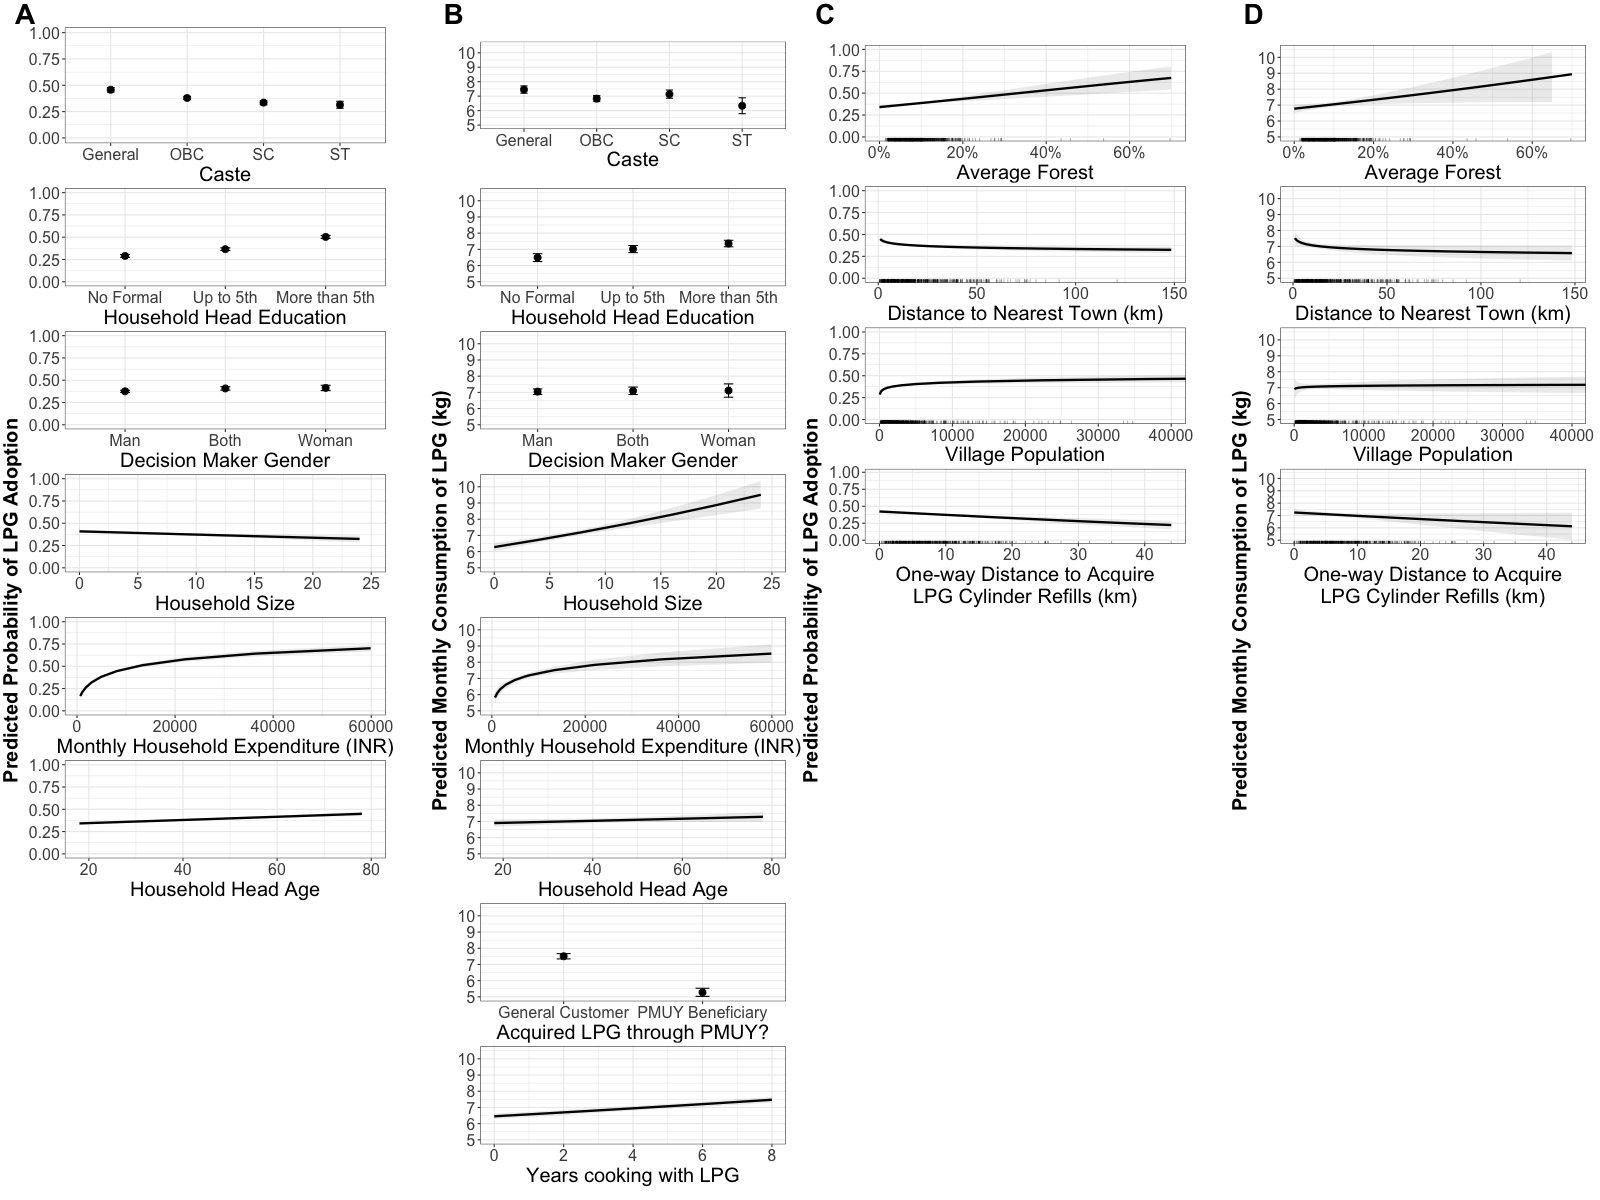
\includegraphics[scale=0.30]{Figures/Marginal_Effects/churdle_ME_village.png}
	\caption{\textbf{Average adjusted predictions of LPG selection and consumption from two-stage double-hurdle model with village-level covariates.}  \textbf{A.} The left panel shows the average-adjusted predicted probability of LPG adoption between 0 and 1 in the model's first stage with 95\% confidence intervals. \textbf{B.} The right panel shows the average-adjusted prediction of monthly consumption -- on condition of LPG adoption -- in kilograms in the model's second stage. Panels \textbf{C.} and \textbf{D.} repeat the same for the village-level covariates. Standard errors in the both model stages are clustered by village.} 
	\label{churdle_ME_village}
\end{figure}

%\begin{figure}[h!]
%\centering
%\includegraphics[scale=1]{Figures/Marginal_Effects/churdle_selection.pdf}
%\caption{Marginal Effects of Double Hurdle Model (First Stage: Selection). This figure shows an average marginal effect of significant variables in predicting LPG selection with a 95\% of confidence level. }
%\label{churdle_selection}
%\end{figure}

%\begin{figure}[h!]
%\centering
%\includegraphics[scale=1]{Figures/Marginal_Effects/churdle_consumption.pdf}
%\caption{Marginal Effects of Double Hurdle Model (Second Stage: Consumption). This figure shows an average marginal effect of significant variables in predicting LPG consumption with a 95\% of confidence level.}
%\label{churdle_consumption}
%\end{figure}


\section{Supplementary Tables}
\label{sect:additional}


\begin{table}
\centering
\renewcommand{\arraystretch}{1.5}

% Table created by stargazer v.5.2.2 by Marek Hlavac, Harvard University. E-mail: hlavac at fas.harvard.edu
% Date and time: Fri, Jul 10, 2020 - 10:45:18 AM
\begin{tabular}{@{\extracolsep{5pt}} cccccc} 
\\[-1.8ex]\hline 
\hline \\[-1.8ex] 
 & Mean & SD & Min & Max & Observations \\ 
\hline \\[-1.8ex] 
LPG (1 = yes, 0 = no) & $0.212$ & $0.409$ & $0$ & $1$ & 8,518 \\ 
LPG Exclusive Use & $0.043$ & $0.203$ & $0$ & $1$ & 8,518 \\ 
Fuel Stacking with LPG as Primary & $0.080$ & $0.271$ & $0$ & $1$ & 8,518 \\ 
Fuel Stacking with Other Fuels as Primary & $0.089$ & $0.285$ & $0$ & $1$ & 8,518 \\ 
No Adoption of LPG & $0.788$ & $0.409$ & $0$ & $1$ & 8,518 \\ 
\hline \\[-1.8ex] 
\end{tabular} 

\caption{Summary Statistics of Dependent Variables (2015)}
\label{t:sum_dependent_2015}
\end{table}

\begin{table}
\centering
\renewcommand{\arraystretch}{1.5}

% Table created by stargazer v.5.2.2 by Marek Hlavac, Harvard University. E-mail: hlavac at fas.harvard.edu
% Date and time: Fri, Jul 10, 2020 - 10:45:31 AM
\begin{tabular}{@{\extracolsep{5pt}} cccccc} 
\\[-1.8ex]\hline 
\hline \\[-1.8ex] 
 & Mean & SD & Min & Max & Observations \\ 
\hline \\[-1.8ex] 
LPG (1 = yes, 0 = no) & $0.533$ & $0.499$ & $0$ & $1$ & 8,797 \\ 
LPG Exclusive Use & $0.155$ & $0.362$ & $0$ & $1$ & 8,797 \\ 
Fuel Stacking with LPG as Primary & $0.160$ & $0.367$ & $0$ & $1$ & 8,797 \\ 
Fuel Stacking with Other Fuels as Primary & $0.217$ & $0.412$ & $0$ & $1$ & 8,797 \\ 
No Adoption of LPG & $0.467$ & $0.499$ & $0$ & $1$ & 8,797 \\ 
\hline \\[-1.8ex] 
\end{tabular} 

\caption{Summary Statistics of Dependent Variables (2018)}
\label{t:sum_dependent_2018}
\end{table}

\begin{table}
\centering
\renewcommand{\arraystretch}{1.5}

% Table created by stargazer v.5.2.2 by Marek Hlavac, Harvard University. E-mail: hlavac at fas.harvard.edu
% Date and time: Fri, Jul 10, 2020 - 11:25:10 AM
\begin{tabular}{@{\extracolsep{5pt}} cccccc} 
\\[-1.8ex]\hline 
\hline \\[-1.8ex] 
 & Mean & SD & Min & Max & Observations \\ 
\hline \\[-1.8ex] 
log (Monthly Expenditure) & $8.390$ & $0.599$ & $6$ & $10$ & 8,518 \\ 
Monthly Expenditure & $5,300$ & $3,900$ & $500$ & $60,000$ & 8,518 \\ 
Household Size & $6.740$ & $3.540$ & $1$ & $50$ & 8,518 \\ 
Caste: SC & $0.184$ & $0.387$ & $0$ & $1$ & 8,518 \\ 
Caste: ST & $0.101$ & $0.301$ & $0$ & $1$ & 8,518 \\ 
Caste: OBC & $0.476$ & $0.499$ & $0$ & $1$ & 8,518 \\ 
Caste: General & $0.239$ & $0.427$ & $0$ & $1$ & 8,518 \\ 
Edu: NoFormalSchooling & $0.320$ & $0.466$ & $0$ & $1$ & 8,518 \\ 
Edu:UpTo5thStandard & $0.310$ & $0.462$ & $0$ & $1$ & 8,518 \\ 
Edu:MoreThan5thStandard & $0.370$ & $0.483$ & $0$ & $1$ & 8,518 \\ 
Religion:Hindu & $0.872$ & $0.334$ & $0$ & $1$ & 8,518 \\ 
Religion:Other & $0.128$ & $0.334$ & $0$ & $1$ & 8,518 \\ 
Decision Maker Age & $42.300$ & $14.200$ & $20$ & $100$ & 8,518 \\ 
Man Decision Maker & $0.780$ & $0.415$ & $0$ & $1$ & 8,518 \\ 
Women Decision Maker & $0.057$ & $0.232$ & $0$ & $1$ & 8,518 \\ 
Both Gender & $0.164$ & $0.370$ & $0$ & $1$ & 8,518 \\ 
\hline \\[-1.8ex] 
\end{tabular} 

\caption{Summary Statistics of Independent Variables (2015)}
\label{t:sum_indep_2015}
\end{table}

\begin{table}
\centering
\renewcommand{\arraystretch}{1.5}

% Table created by stargazer v.5.2.2 by Marek Hlavac, Harvard University. E-mail: hlavac at fas.harvard.edu
% Date and time: Fri, Jul 10, 2020 - 11:25:24 AM
\begin{tabular}{@{\extracolsep{5pt}} ccccccc} 
\\[-1.8ex]\hline 
\hline \\[-1.8ex] 
 & Mean & SD & Min & Max & NA & Observations \\ 
\hline \\[-1.8ex] 
log (Monthly Expenditure) & $8.555$ & $0.640$ & $0$ & $10$ & $60$ & 8,797 \\ 
Monthly Expenditure & $6,285.527$ & $8.555$ & $0$ & $80,000$ & $60$ & 8,797 \\ 
Household Size & $6.195$ & $3.221$ & $1$ & $40$ & $0$ & 8,797 \\ 
Caste: SC & $0.194$ & $0.396$ & $0$ & $1$ & $0$ & 8,797 \\ 
Caste: ST & $0.108$ & $0.310$ & $0$ & $1$ & $0$ & 8,797 \\ 
Caste: OBC & $0.468$ & $0.499$ & $0$ & $1$ & $0$ & 8,797 \\ 
Caste: General & $0.230$ & $0.421$ & $0$ & $1$ & $0$ & 8,797 \\ 
Edu: NoFormalSchooling & $0.389$ & $0.488$ & $0$ & $1$ & $0$ & 8,797 \\ 
Edu:UpTo5thStandard & $0.308$ & $0.462$ & $0$ & $1$ & $0$ & 8,797 \\ 
Edu:MoreThan5thStandard & $0.303$ & $0.460$ & $0$ & $1$ & $0$ & 8,797 \\ 
Religion:Hindu & $0.880$ & $0.324$ & $0$ & $1$ & $0$ & 8,797 \\ 
Religion:Other & $0.120$ & $0.324$ & $0$ & $1$ & $0$ & 8,797 \\ 
Decision Maker Age & $43.220$ & $14.820$ & $20$ & $100$ & $0$ & 8,797 \\ 
Man Decision Maker & $0.669$ & $0.471$ & $0$ & $1$ & $0$ & 8,797 \\ 
Women Decision Maker & $0.069$ & $0.254$ & $0$ & $1$ & $0$ & 8,797 \\ 
Both Gender & $0.262$ & $0.440$ & $0$ & $1$ & $0$ & 8,797 \\ 
\hline \\[-1.8ex] 
\end{tabular} 

\caption{Summary Statistics of Independent Variables (2018)}
\label{t:sum_indep_2018}
\end{table}

\begin{table}
\centering
\renewcommand{\arraystretch}{1.5}
\resizebox{\columnwidth}{!}{%
\def\sym#1{\ifmmode^{#1}\else\(^{#1}\)\fi}
\begin{tabular}{l*{5}{c}}
\hline\hline
                    &\multicolumn{2}{c}{(1)}                              &\multicolumn{3}{c}{(2)}                                           \\
                    &\multicolumn{2}{c}{Two-Stage Model}                        &\multicolumn{3}{c}{Generalized Ordered Logit Model}  \\
                    &  Consumption         &Selection         &  No LPG         &No LPG        &  No LPG \&\\
                    &          &         &          &\& Stacking     &   Stacking (LPG Secondary) \\
                    &   &     &        & (LPG Secondary)     &  \& Stacking (LPG Primary)\\       
                    
\hline
log (Monthly Expenditure)&       0.146\sym{***}&       0.430\sym{***}&        0.521\sym{***}&       0.543\sym{***}&       0.491\sym{***}\\
                    &    (0.0152)         &    (0.0234)        &    (0.0254)         &    (0.0223)         &    (0.0182)         \\
[1em]
Household Size       &       0.0132\sym{***}&     -0.0152\sym{***}&       1.080\sym{***}&       1.042\sym{***}&       1.025\sym{***}\\
                    &    (0.00253)         &   (0.00374)        &    (0.0120)         &   (0.00791)         &   (0.00634)         \\
[1em]
Education: Up to 5th Standard          &       0.120\sym{***}&       0.275\sym{***}&              0.670\sym{***}&       0.596\sym{***}&       0.625\sym{***}\\
                    &    (0.0223)         &    (0.0279)            &    (0.0433)         &    (0.0299)         &    (0.0285)         \\
[1em]                    
Education: More than 5th Standard         &        0.231\sym{***}&       0.700\sym{***}&      0.321\sym{***}&       0.321\sym{***}&       0.321\sym{***}\\
                    &    (0.0211)         &    (0.0319)       &    (0.0159)         &    (0.0159)         &    (0.0159)         \\
[1em]
Caste: OBC             &     -0.0968\sym{***}&      -0.235\sym{***}&              1.488\sym{***}&       1.488\sym{***}&       1.488\sym{***}\\
                    &    (0.0212)         &    (0.0370)         &     (0.0855)         &    (0.0855)         &    (0.0855)         \\
[1em]
Caste: ST            &      -0.218\sym{***}&      -0.509\sym{***} &     2.192\sym{***}&       2.192\sym{***}&       2.192\sym{***}\\
                    &    (0.0531)         &    (0.0682)         &   (0.256)         &     (0.256)         &     (0.256)         \\
[1em]
Caste: SC             &      -0.133\sym{***}&      -0.362\sym{***}&    1.773\sym{***}&       1.773\sym{***}&       1.773\sym{***}\\
                    &    (0.0268)         &    (0.0452)         &     (0.125)         &     (0.125)         &     (0.125)         \\                 
[1em]
Gender: Woman   &      0.0374         &       0.192\sym{***} &       0.734\sym{***}&       0.734\sym{***}&       0.734\sym{***}\\
                   &    (0.0298)         &    (0.0480)      &    (0.0536)         &    (0.0536)         &    (0.0536)        \\
[1em]
Gender: Both          &      0.0298         &       0.118\sym{***}  &         0.865\sym{*}  &       0.766\sym{***}&       0.804\sym{***}\\
                    &     (0.0187)         &    (0.0292)         &    (0.0600)         &    (0.0398)         &    (0.0376)       \\
[1em]
Religion: Hindu        &     -0.0620\sym{*}  &      0.0371           &        1.067         &       1.099         &       0.950        \\
                    &    (0.0313)         &    (0.0527)         &    (0.114)         &     (0.106)         &    (0.0836)         \\
[1em]
Decision Maker Age          &     0.00196\sym{***}&     0.00553\sym{***}&       0.991\sym{***}&       0.991\sym{***}&       0.991\sym{***}\\
                    &  (0.000546)         &  (0.000813)         &   (0.00125)         &   (0.00125)         &   (0.00125)         \\
\hline\hline
\multicolumn{6}{l}{\footnotesize Standard errors in parentheses, clustered by village}\\
\multicolumn{6}{l}{\footnotesize \sym{*} \(p<0.05\), \sym{**} \(p<0.01\), \sym{***} \(p<0.001\)}\\
\end{tabular}%
}
\caption{Double hurdle model (1) and generalized ordered logit model (2). This table shows the regression results from our two main models. Coefficients in model (1) show the impact of variables on the two stages of LPG selection and consumption. Coefficients in model (2) show the impact of variables on three combined outcomes of LPG adoption. The coefficients for model (2) have been converted to odds ratio. We use relaxed parallel assumptions on household size, education of more than 5th standard, and caste of ST in generalized ordered logit model.}
\label{t:gologit&hurdle}
\end{table}

\begin{table}
\centering
\renewcommand{\arraystretch}{1.5}
\resizebox{\columnwidth}{!}{%
\def\sym#1{\ifmmode^{#1}\else\(^{#1}\)\fi}
\begin{tabular}{l*{5}{c}}
\hline\hline
                    &\multicolumn{2}{c}{(1)}                              &\multicolumn{3}{c}{(2)}                                           \\
                    &\multicolumn{2}{c}{Two-Stage Model}                        &\multicolumn{3}{c}{Generalized Ordered Logit Model}  \\
                    &  Consumption         &Selection         &  No LPG         &No LPG        &  No LPG \&\\
                    &          &         &          &\& Stacking     &   Stacking (LPG Secondary) \\
                    &   &     &        & (LPG Secondary)     &  \& Stacking (LPG Primary)\\       
                    
\hline
pmuy                 &      -0.351\sym{***}&                     &                     &                     &                     \\
                    &    (0.0248)         &                     &                     &                     &                     \\
[1em]
log (Monthly Expenditure)&      0.0850\sym{***}&       0.427\sym{***}&       0.577\sym{***}&       0.585\sym{***}&       0.511\sym{***}\\
                    &    (0.0145)         &    (0.0314)         &    (0.0300)         &    (0.0251)         &    (0.0199)         \\
[1em]
Household Size       &      0.0173\sym{***}&     -0.0107\sym{*}  &       1.079\sym{***}&       1.043\sym{***}&       1.022\sym{**} \\
                    &   (0.00259)         &   (0.00487)         &    (0.0139)         &   (0.00869)         &   (0.00670)         \\
[1em]
Education: Up to 5th Standard           &      0.0782\sym{***}&       0.293\sym{***}&       0.640\sym{***}&       0.640\sym{***}&       0.640\sym{***}\\
                     &    (0.0225)         &    (0.0434)         &    (0.0304)         &    (0.0304)         &    (0.0304)         \\
[1em]
Education: More than 5th Standard      &       0.126\sym{***}&       0.804\sym{***}&          0.329\sym{***}&       0.329\sym{***}&       0.329\sym{***}\\
                    &    (0.0216)         &    (0.0481)         &    (0.0176)         &    (0.0176)         &    (0.0176)         \\
[1em]
Caste: OBC             &     -0.0878\sym{***}&      -0.296\sym{***}&       1.522\sym{***}&       1.522\sym{***}&       1.522\sym{***}\\
                   &    (0.0216)         &    (0.0476)           &    (0.0899)         &    (0.0899)         &    (0.0899)         \\
[1em]
Caste: ST         &      -0.163\sym{***}&      -0.488\sym{***} &       2.068\sym{***}&       2.068\sym{***}&       2.068\sym{***}\\
                    &    (0.0464)         &    (0.0819)         &     (0.229)         &     (0.229)         &     (0.229)         \\
Caste: SC             &     -0.0434         &      -0.573\sym{***} &       1.879\sym{***}&       1.879\sym{***}&       1.879\sym{***}\\
                     &    (0.0267)         &    (0.0654)       &     (0.144)         &     (0.144)         &     (0.144)         \\
[1em]
Gender: Woman   &     0.00969         &       0.212\sym{**}  &       0.819\sym{**} &       0.819\sym{**} &       0.819\sym{**} \\
                   &    (0.0300)         &    (0.0709)         &    (0.0600)         &    (0.0600)         &    (0.0600)         \\
[1em]
Gender: Both          &     0.00734         &       0.127\sym{**}  &       0.920         &       0.787\sym{***}&       0.811\sym{***}\\
                   &    (0.0182)         &    (0.0471)         &    (0.0680)         &    (0.0445)         &    (0.0414)         \\
[1em]
Religion: Hindu         &     -0.0756\sym{*}  &       0.184\sym{**}         &       1.008         &       1.020         &       0.847         \\
                    &    (0.0306)         &    (0.0614)        &     (0.111)         &    (0.0982)         &    (0.0725)         \\
[1em]
Decision Maker Age             &    0.000908         &     0.00652\sym{***}&       0.991\sym{***}&       0.991\sym{***}&       0.991\sym{***}\\
                    &  (0.000516)         &   (0.00113)         &   (0.00134)         &   (0.00134)         &   (0.00134)         \\
[1em]
LPG Connection Years &      0.0183\sym{***}&                     &                     &                     &                     \\
                    &   (0.00194)         &                     &                     &                     &                     \\
[1em]
Village Average Forest           &     0.00396\sym{*}  &      0.0174\sym{***}&       0.974\sym{***}&       0.974\sym{***}&       0.974\sym{***}\\
                    &   (0.00165)         &   (0.00435)         &   (0.00603)         &   (0.00603)         &   (0.00603)         \\
[1em]
log (Village Population)      &     0.00615         &       0.129\sym{***}&       0.864\sym{***}&       0.864\sym{***}&       0.864\sym{***}\\
                    &    (0.0133)         &    (0.0271)         &    (0.0313)         &    (0.0313)         &    (0.0313)         \\
[1em]
Village LPG Distance &    -0.00380         &     -0.0139\sym{**} &       1.005         &       1.023\sym{**} &       1.025\sym{***}\\
                    &   (0.00242)         &   (0.00455)         &    (0.0102)         &   (0.00791)         &   (0.00677)         \\
[1em]
log (Village Town Distance) &     -0.0268\sym{*}  &     -0.0971\sym{***}&       1.138\sym{**} &       1.138\sym{**} &       1.138\sym{**} \\
                    &    (0.0136)         &    (0.0294)         &    (0.0471)         &    (0.0471)         &    (0.0471)         \\
[1em]
\hline\hline
\multicolumn{6}{l}{\footnotesize Standard errors in parentheses, clustered by village}\\
\multicolumn{6}{l}{\footnotesize \sym{*} \(p<0.05\), \sym{**} \(p<0.01\), \sym{***} \(p<0.001\)}\\
\end{tabular}%
}
\caption{Double hurdle model (1) and generalized ordered logit model (2) with three village-level covariates added: distance to nearest town in kilometers (logged, 2001 Census), village population (logged, 2011 Census), and average distance to LPG source in kilometers (among LPG users only). } 
\label{t:gologit&hurdle_app_full}
\end{table}

\clearpage

\bibliographystyle{naturemag}
\bibliography{../cooking}

\end{document}